\section{Experiment Methodology} \label{sec:methodology}
    Here, we present some preliminary findings in an experiment to meant to investigate whether \xQ{} and \xO{} have effects on user behavior and perception. In order to do this we designed an Amazon Mechanical Turk experiment where human users acted as dispatch supervisors of the unmanned delivery truck described in Sec.~\ref{sec:donut_delivery}. They key hypothesis is that users who are presented with self-confidence metrics will perform better in the dispatch task which will be reflected in a higher score (discussed in detail in Sec.~\ref{sec:hyp_sec_meas}).

    The responsibility of each participant was to decide whether the autonomous delivery vehicle should attempt to make a delivery, or decline the delivery. A successful attempt resulted in +1 point, failure in -1 point, and declining a delivery in -1/4 point. After being trained the participants saw a sequence of 43 different delivery scenarios with varying maps. The experiment was a between-subjects design with 4 conditions. The first condition was the control condition where the users only had the map to use to make decisions. In condition 2 users were presented with \xQ{}, and in condition 3 they were shown \xO. In condition 4 users were given both \xQ{} and \xO. A screenshot of a typical task is shows in Fig.~\ref{fig:screenshot}. Based on feedback from a pilot study the numerical values for \xQ{} and \xP{} were subdivided into regions and converted to words such as `very good' or `bad' as detailed in Tab.~\ref{tab:word_ranges} to help users more easily grasp the scales.

       \begin{figure}[tb]
            \centering
            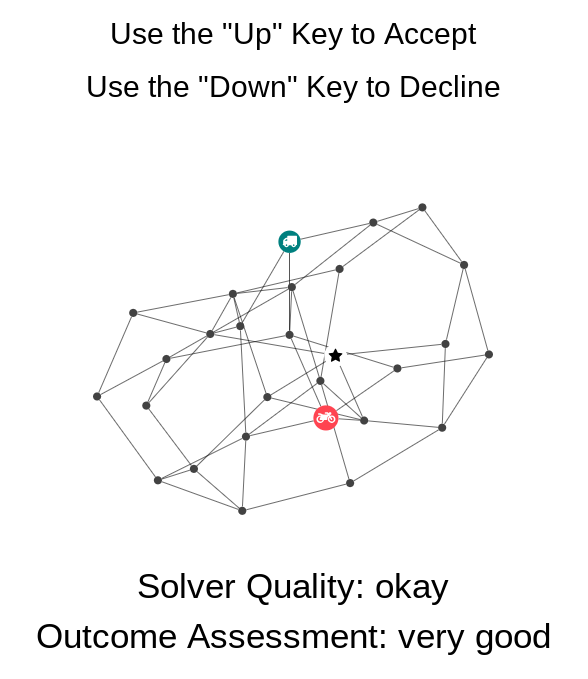
\includegraphics[width=0.8\linewidth]{Figures/experiment_screenshot}
            \caption{Experiment Screenshot}
            \label{fig:screenshot}
        \end{figure}

    The total number of participants represented is N=257, with $n=\{63,63,64,65\}$ for conditions 1-4 respectively. The results of two participants were not included because of inability to follow the instructions satisfactorily. Participants were paid a base rate of $\$1.60$ for the Human Intelligence Task (HIT), and were able to get a bonus of up to $\$1.00$ based on their performance. Pilot data indicated that this would be equivalent to approximately \$7-10/hr. In practice the Turkers were quite a bit faster than those in the pilot study, and earned around \$13/hr.

    \subsubsection{Hypotheses, Conditions, and Measures} \label{sec:hyp_cond_meas}
    \paragraph{Experiment Variables:}
    The two \famsec{} metrics discussed herein are the experimental variables in this situation, each will be either `present' or `absent'. Therefore this study is a 2(\xQ) $\times$ 2(\xO) design, resulting in 4 conditions:

    \begin{enumerate}[label=\textbf{C\arabic*}]
        \item (Control): The participant will make decisions based solely on information provided by the visualization of the task. They will still receive feedback about success/failure. \label{itm:C1}
        \item The participant will make decisions on the same tasks as in the control, but with \xQ{} displayed as well.\label{itm:C2}
        \item The participant will make decisions on the same tasks as in the control, but with \xO{} as well. \label{itm:C3}
        \item The participant will make decisions on the same tasks as in the control, but with both \xQ{}, and \xO{} displayed simultaneously. \label{itm:C4}
    \end{enumerate}

    The experiment was designed to investigate five main hypotheses. Generally, the overarching hypotheses is that \xQ{} and \xO{} have significant effects on user behavior and perception when presented, as opposed to when they are not. Given other similar work in the area of trust between humans and technology (surveyed in \cite{Israelsen2017-ym}) there is reason to believe that this is the case.

    \begin{enumerate}[label=\textbf{H\arabic*}]
        \item Use of either, or both, FaMSeC metrics (\xQ{} and \xO{}) improves performance of the user-autonomy team on the experimental task when compared to control condition. (i.e. presence of FaMSeC metrics will affect the TRBs of human users) \label{itm:H1}
        \item Users who are presented with FaMSeC metrics will rate trust of autonomous system more highly than in control condition. (i.e. presence of FaMSeC metrics will affect the self-reported trust of human users) \label{itm:H2}
        \item Users who are presented with FaMSeC metrics will make decisions about delegation more quickly than those in control condition. (i.e. the presence of FaMSeC will help the user offload some of their workload onto the autonomous system) \label{itm:H3}
        \item Users not in the control condition will rate the ‘quality’ of the AS higher than those in the control \label{itm:H4}
        \item Users not in the control condition will be more willing to work with the system again. \label{itm:H5}
    \end{enumerate}

    \paragraph{Measures:}
    The following measurements were gathered for each participant.
    \begin{enumerate}[label=\textbf{M\arabic*}]
        \item Score---cumulative score of user during experimental tasks. Used for \ref{itm:H1}
        \item Questionnaire Responses---Likert scale responses to survey questions. Used for \ref{itm:H2},\ref{itm:H4}, and \ref{itm:H5}
        \item Average time per task---average time for user to make decision during experimental tasks. Used for \ref{itm:H3}
    \end{enumerate}

    \begin{table}[]
        \caption{Natural Language Prompts Used for Metric Values}
        \label{tab:word_ranges}
        \begin{tabular}{cclcc}
            \multicolumn{2}{c}{\xQ{}} & \vline & \multicolumn{2}{c}{\xO{}} \\
            Range & Prompt & \vline & Range & Prompt \\
            \hline
            $[0.00,0.40]$ & Very Bad & \vline & $[-1.0,-0.5]$ & Very Bad \\
            $(0.40,0.75]$ & Bad & \vline & $(-0.5,-0.10]$ & Bad \\
            $(0.75,1.00]$ & Okay & \vline & $(-0.10,0.10]$ & Okay \\
            $(1.00,1.50]$ & Good & \vline & $(0.10,0.50]$ & Good \\
            $(1.50,2.00]$ & Very Good & \vline & $(0.50,1.00]$ & Very Good
        \end{tabular}
    \end{table}
